\section{Cahn-Hilliard Phase Decomposition}

%%%%%%%%%%%%%%%%%%%%%%%%%%%%%%%%%%%%%%%%%%%%%%%%%%%%%%%%%%%%%%%%%%%%%
\royslide{Microscale and Nanoscale Applications}{
Cahn-Hilliard phase decomposition can model such disparate phenomena
as:
\royitemizebegin
\item Tin-Lead solder aging
\item Void lattice formation in irradiated semiconductors
\item Self-assembly of thin film patterns
\royitemizeend

\begin{center}
%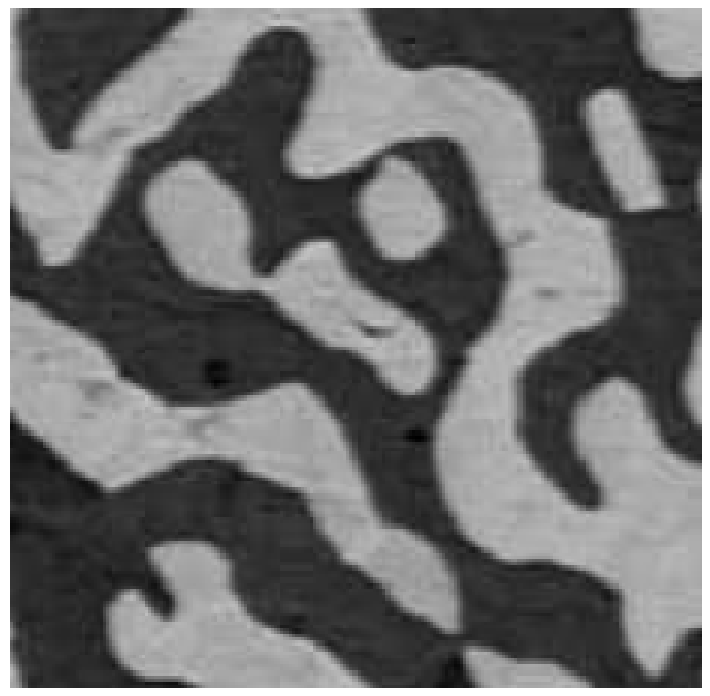
\includegraphics[width=.3\textwidth]{figs/PbSb}
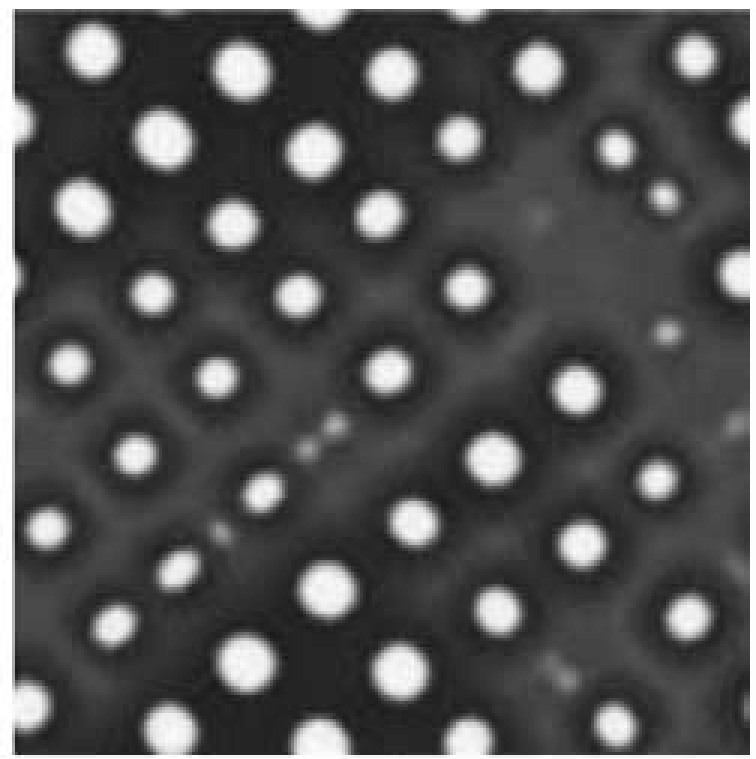
\includegraphics[width=.3\textwidth]{figs/nanovoids}
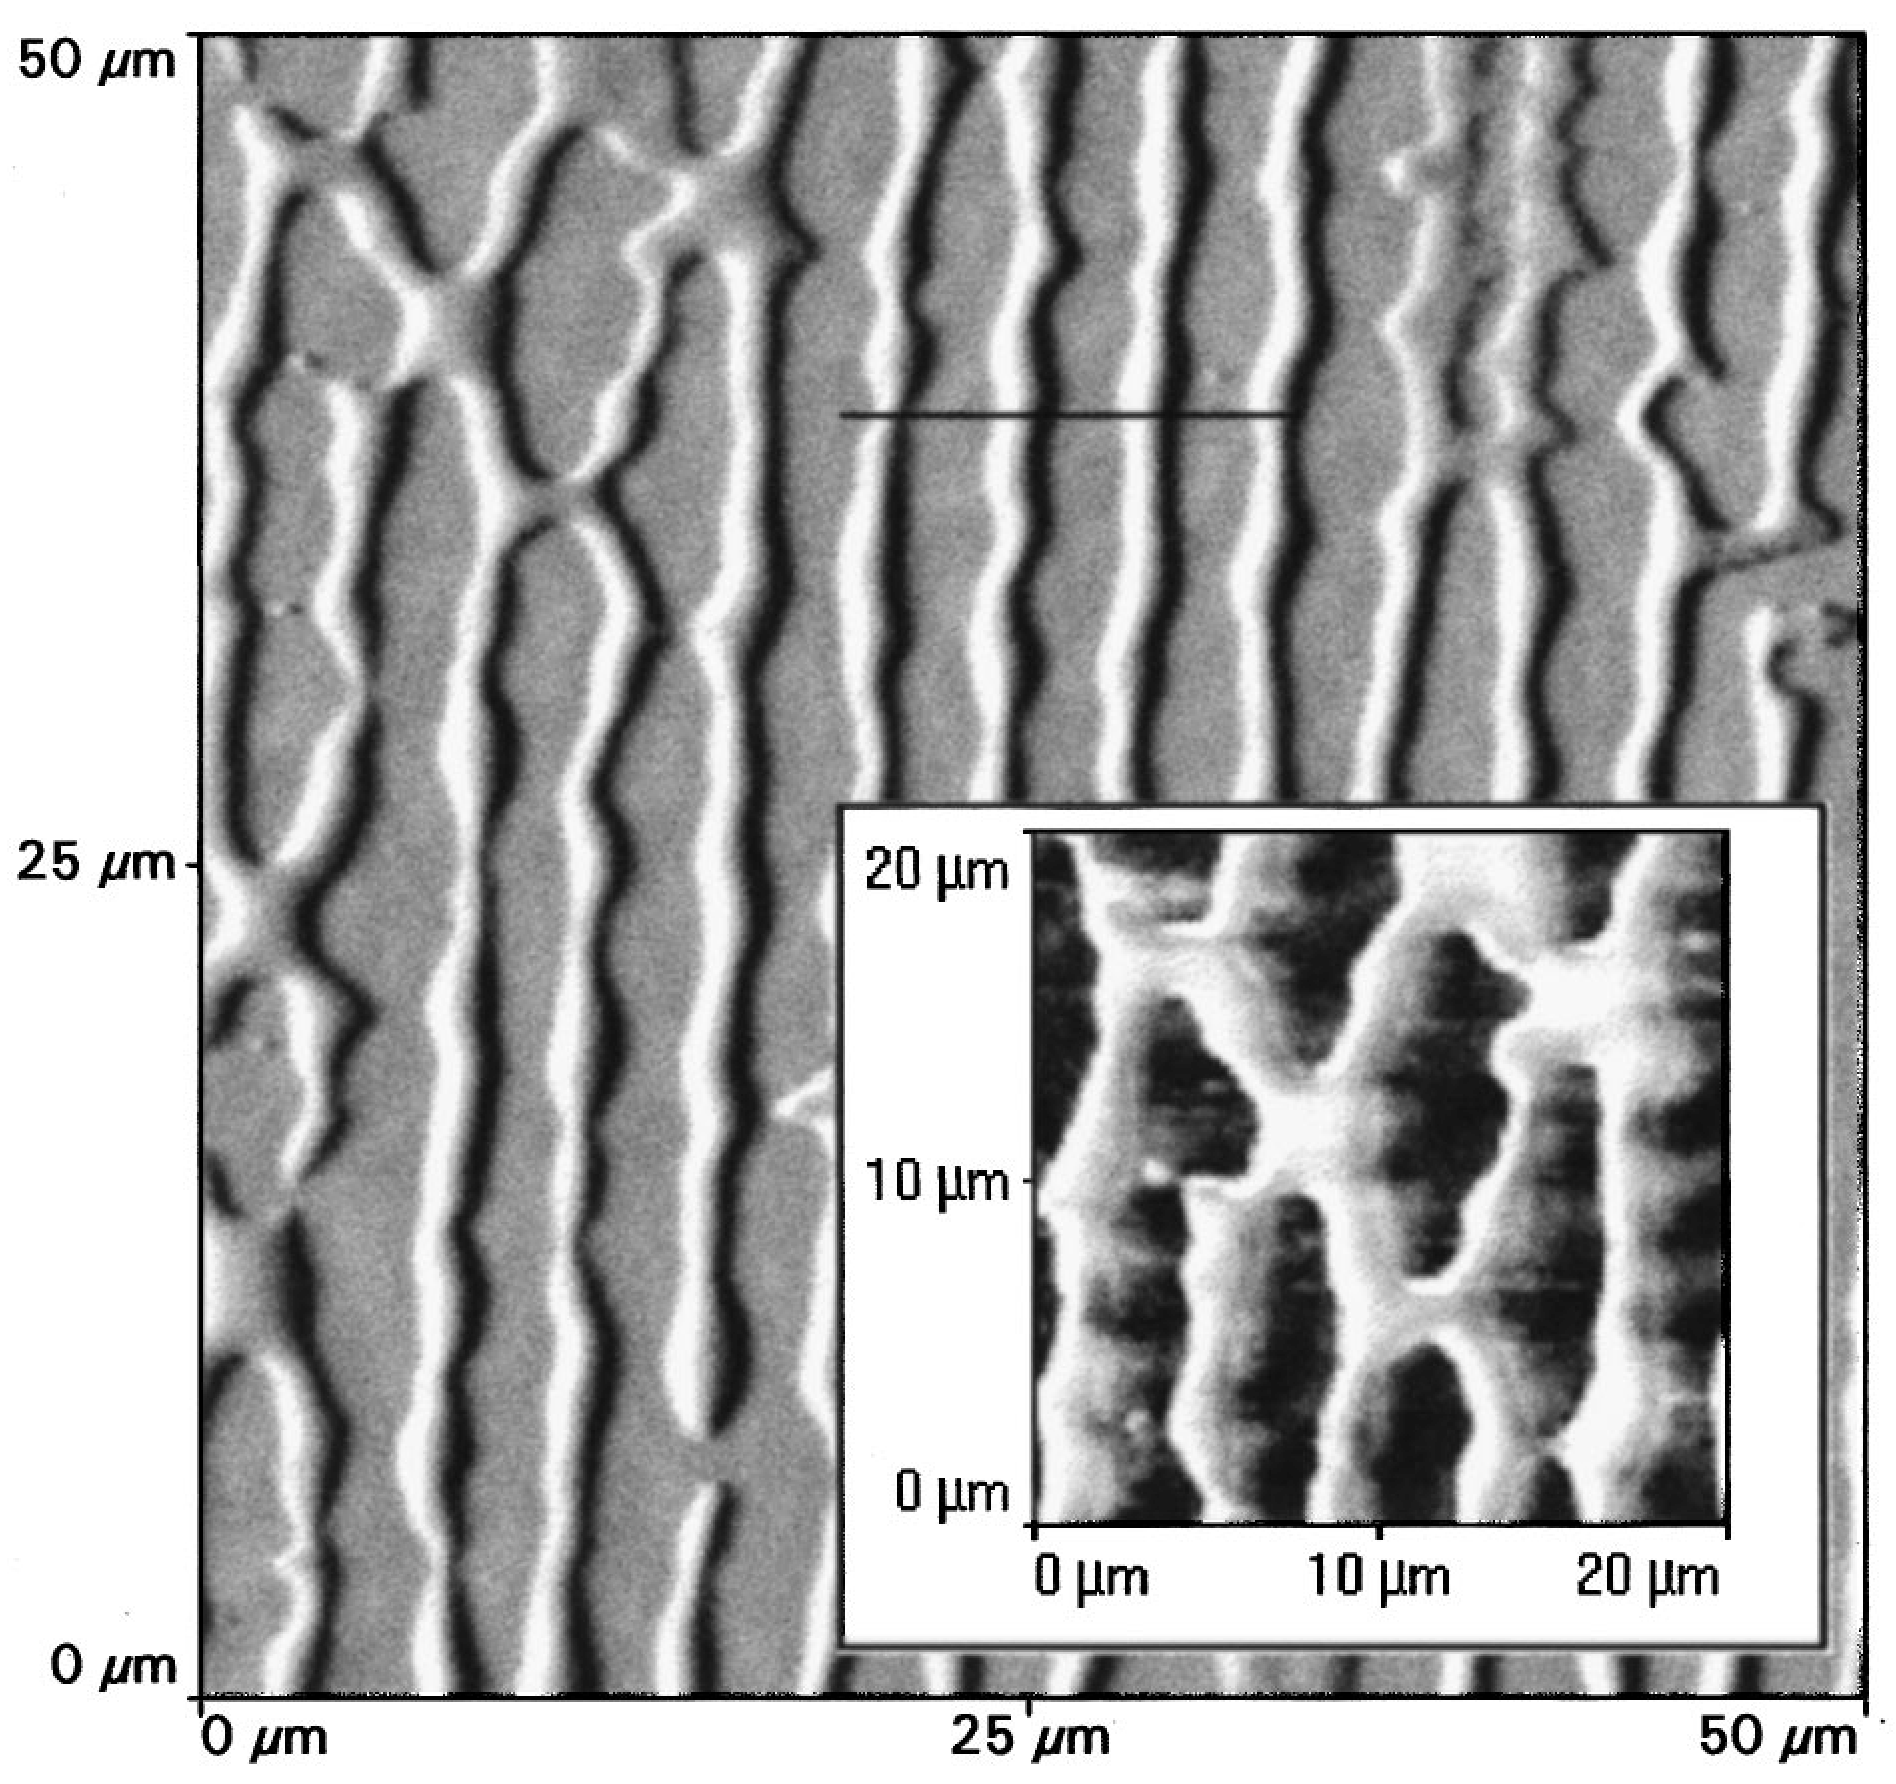
\includegraphics[width=.3\textwidth]{figs/polymer-pattern}
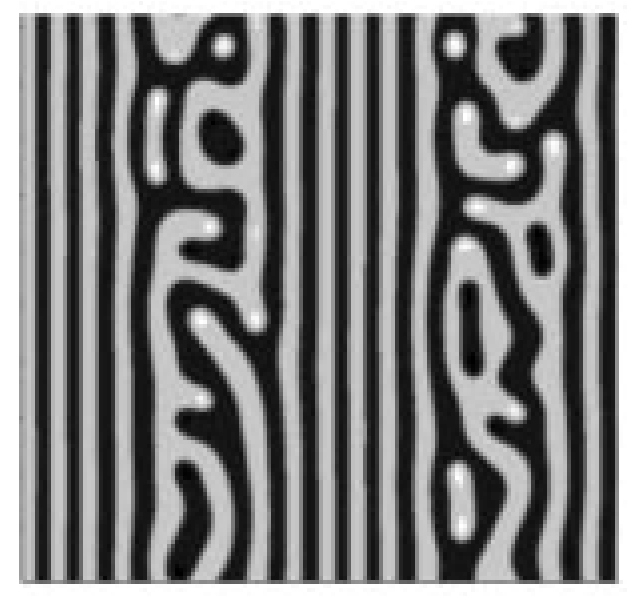
\includegraphics[width=.3\textwidth]{figs/programmedpattern}
\end{center}

}


%%%%%%%%%%%%%%%%%%%%%%%%%%%%%%%%%%%%%%%%%%%%%%%%%%%%%%%%%%%%%%%%%%%%%
\royslide{Free Energy Formulation}{

Cahn-Hilliard systems model material separation and interface
evolution by tracking flow driven by configurational and interfacial
free energy minimization.

\begin{minipage}[h]{.45\textwidth}
\begin{eqnarray*}
f_0(c) & \equiv & \frac{1}{4} \left( c^2 - 1 \right)^2 \\
f_\gamma(\nabla c) & \equiv & \frac{\epsilon_c^2}{2} \nabla c \cdot
\nabla c
\end{eqnarray*}
\end{minipage}
\begin{minipage}[h]{.45\textwidth}
\includegraphics[width=.9\textwidth]{figs/doublewell}
\end{minipage}

}


%%%%%%%%%%%%%%%%%%%%%%%%%%%%%%%%%%%%%%%%%%%%%%%%%%%%%%%%%%%%%%%%%%%%%
\royslide{Cahn-Hilliard Equation}{

Adding a material-dependent mobility coefficient defines the
concentration flux.

\begin{eqnarray*}
\vec{J} & = & M_c \nabla \frac{df}{dc} \\
  & = & M_c \nabla \left( f_0'(c) + f_\gamma'(c) \right) \\
  & = & M_c \nabla \left( c^3 - c - \epsilon_c^2 \Laplacian c \right)
\end{eqnarray*}

\begin{eqnarray*}
\dt{c} & = & \nabla \cdot M_c \nabla
  \left( c^3 - c - \epsilon_c^2 \Laplacian c \right)
\end{eqnarray*}

}


%%%%%%%%%%%%%%%%%%%%%%%%%%%%%%%%%%%%%%%%%%%%%%%%%%%%%%%%%%%%%%%%%%%%%
\royslide{Weak Cahn-Hilliard Equation}{

Taking a weighted residual and integrating by parts twice,

\begin{eqnarray*}
(\dt{c},\phi)_\Omega & = & - \left(M_c \nabla \left( c^3 - c \right),
                \nabla \phi \right)_\Omega - \epsilon_c^2
                \left( \Laplacian c, \nabla \cdot M_c^T \nabla \phi
\right)_\Omega
\nonumber \\
  &   & + \left(\left(M_c \nabla \left( c^3 - c -
          \epsilon_c^2 \Laplacian c\right) \right) \cdot \vec{n},
          \phi \right)_{\partial \Omega} \\
  &   & + \epsilon_c^2 \left( \Laplacian c, M_c^T \nabla \phi \cdot
\vec{n} \right)_{\partial \Omega}
\end{eqnarray*}

Gives a functional defined on $W^{2,2}(\Omega) \cap W^{1,4}(\Omega)$
in case of constant $M_c$.

}


